% -----------------------------------------------
% Template for ISMIR Papers
% 2018 version, based on previous ISMIR templates

% Requirements :
% * 6+n page length maximum
% * 4MB maximum file size
% * Copyright note must appear in the bottom left corner of first page
% * Clearer statement about citing own work in anonymized submission
% (see conference website for additional details)
% -----------------------------------------------

\documentclass{article}
\usepackage{ismir,amsmath,cite,url}
\usepackage{graphicx}
\usepackage{color}
\usepackage[usenames, table]{xcolor}
\usepackage{subcaption}
% \usepackage[table]
\newcommand {\ad}[1]{{\color{blue}{[{#1}]}}}
\newcommand {\aj}[1]{{\color{purple}{[AJ] {#1}}}}
\newcommand {\ak}[1]{{\color{teal}{{#1}}}}
\newcommand {\rmb}[1]{{\color{red}{[{#1}]}}}
\newcommand \REDACTED{{\color{orange}{[REDACTED] }}}

% Title.
% ------
\title{Vocals in Music Matter: the Relevance of Vocals in the Minds of Listeners}

% Note: Please do NOT use \thanks or a \footnote in any of the author markup

% Single address
% To use with only one author or several with the same address
% ---------------
\oneauthor
{Andrew Demetriou$^{1,2}$ \hspace{1cm} Andreas Jansson$^2$ \hspace{1cm} Aparna Kumar$^2$ \hspace{1cm} Rachel M. Bittner$^2$}
{ $^1$ Multimedia Computing Group, TU Delft, The Netherlands\\
 $^2$ Spotify Inc., New York City, USA}
\def\authorname{Andrew Demetriou, Andreas Jansson, Aparna Kumar, Rachel M. Bittner}

% Two addresses
% --------------
%\twoauthors
%  {First author} {School \\ Department}
%  {Second author} {Company \\ Address}

%% To make customize author list in Creative Common license, uncomment and customize the next line
%  \def\authorname{First Author, Second Author}


% Three addresses
% --------------
% \threeauthors
%   {First Author} {Affiliation1 \\ {\tt author1@ismir.edu}}
%   {Second Author} {\bf Retain these fake authors in\\\bf submission to preserve the formatting}
%   {Third Author} {Affiliation3 \\ {\tt author3@ismir.edu}}

%% To make customize author list in Creative Common license, uncomment and customize the next line
%  \def\authorname{First Author, Second Author, Third Author}

% Four or more addresses
% OR alternative format for large number of co-authors
% ------------
% \multauthor
% {Andrew Demetriou$^{1,2}$ \hspace{1cm} Andreas Jansson$^2$ \hspace{1cm} Aparna Kumar$^2$ \hspace{1cm} Rachel Bittner$^2$} { } \\
%  $^1$ Multimedia Computing Group, TU Delft, The Netherlands\\
% $^2$ Spotify Inc., New York City, USA\\
% {\tt\small CorrespondenceAuthor@ismir.edu, PossibleOtherAuthor@ismir.edu}}
% \def\authorname{First author, Second author, Third author, Fourth author, Fifth author, Sixth author}


\sloppy % please retain sloppy command for improved formatting

\begin{document}

\maketitle

\begin{abstract}
In music information retrieval, we often make assertions about what features of music are important to study, one of which is vocals.
While the importance of vocals in music preference is both intuitive and anticipated by psychological theory, we have not found any survey studies that confirm this commonly held assertion.
We address two questions: (1) what components of music are most salient to people's musical taste, and (2) how do vocals rank relative to other components of music, in regards to whether people like or dislike a song. Lastly, we explore the aspects of the voice that listeners find important.  Two surveys of Spotify users were conducted. The first gathered open-format responses that were then card-sorted into semantic categories by the team of researchers.  The second asked respondents to rank the semantic categories derived from the first survey. Responses indicate that vocals were a salient component in the minds of listeners. Further, vocals ranked high as a self-reported factor for a listener liking or disliking a track, among a statistically significant ranking of musical attributes.
In addition, we open several new interesting problem areas that have yet to be explored in MIR.
\end{abstract}

\section{Introduction}

%\ak{[We could start this paper by asking what is important in music, instead of saying we want to find vocals.]}

%\ak{ However it is unclear to what extent each of these dimensions plays a role in music preference for listeners.  Here, we survey music listeners from an online streaming platform and we ask them what they like in music... }

The Music Information Retrieval (MIR) community has historically focused on content-based understanding of music. The type of content-based analysis studied over time is typically driven by the data available to the task, or the interests of the specific researchers. An alternative motivator could be to study topics that are salient in the minds of listeners, especially with respect to listener's musical preference. Specifically, understanding which attributes of music contribute the most to music preference, and their relative weight, could help guide research efforts. One attribute of music we would expect to be salient in the minds of listeners is the singing voice.

Psychology research anticipates the importance of the human voice as a salient stimulus, and as a component of music in particular.
The human ability to communicate exceeds that of any other species studied thus far, with both speech and singing being cultural universals reliant on vocal production.
It is theorized that the advanced human ability to communicate, discriminate, and to experience emotional responses in vocalizations has allowed for the emergence of music~\cite{juslin2003music}.
Our emotions are often accompanied by involuntary changes in our physiology and nonverbal expressions,  such as facial expressions and vocalizations \cite{porges2001polyvagal}.
Our reactions to the emotional content expressed in the vocals in music may have similar effects. As such, much psychological research has focused on the singing voice even more than speech, due to the precision required to execute and process musical vocalizations \cite{hutchins2013linked}.
This makes musical vocals a well-anticipated candidate for study as a feature of music, as we would expect people to have a sophisticated ability to deliver, empathize with, and process vocal communications.

We would therefore expect that the vocals in music would be an especially salient component, if not the most salient. While a complete review is beyond the scope of this paper, some research is particularly worth noting.
For example, it has been shown that both adults \cite{weiss2012something} and children \cite{weiss2015enhanced} recall melodies more correctly when sung with the voice than when played with instruments.
Hutchins and Moreno \cite{hutchins2013linked} review literature that shows relatively precise perception of pitch in the human voice, yet fewer noticeable pitch errors in the voice relative to musical instruments or synthesized voices \cite{hutchins2012frog}.
Neuroscience studies show specific areas of the brain involved in processing human voices \cite{belin2000voice}.
Although similar regions of the brain are involved in processing both music and voices, there is differential processing of the human voice relative to music \cite{armony2015specificity}.
As such, the human voice may be processed as a uniquely significant sound.

However, while prior research suggests that vocals would be especially relevant to music preference, no study to our knowledge has assessed the importance of the voice in music, relative to other musical components. To address this gap, we test the hypothesis that the voice is as or more important than other musical components across implicit and explicit datasets, using traditional social science techniques, as well as data mining techniques.
First, we mine data available from Spotify, including playlist titles, search data and artist biographies, to test whether terms related to vocals are prevalent.
However, we show that the results of the data mining are inconclusive as to whether or not vocals are salient in the minds of listeners. Specifically, it is not clear whether the vocals can be disentangled from other factors in playlist titles and search queries, such as genre.
For more conclusive results, we gather data from users explicitly. To this aim we conduct two online survey studies: the first gathered subjective data on the salient components of music directly from listener reports, which were separated into semantic categories using card-sorting. The second asked participants to rank the semantic categories from the first study in terms of importance to their musical preference. We conclude that two aspects related to the voice are especially salient, namely the voice itself, and the lyrics of the song. Furthermore, we highlight the importance of gathering explicit data to complement implicit techniques, in situations where factors may not be easily disentangled.

\section{Vocals in Semantic Data}
%From prior research, we might expect that listeners perceive vocals as an important attribute of music.  %% [AJ] repeating ourselves
Prior research has shown that semantic descriptors of music may be an appropriate means for users to query music databases \cite{lesaffre2008potential}. Given the large amount of semantic data available to Spotify such as playlist titles, search results, and artist biographies, one might hypothesize that terms describing the vocals would commonly appear in this implicit data.
%To test this, we examine semantic tags mined from playlist titles, descriptive search queries, and album reviews. %% [AJ] redundant

\subsection{Playlist Tags and Search Queries}
Non-common words or groups of words and emojis appearing in the titles of a large number of Spotify's user-generated playlists were aggregated to create a list of the 1000 most frequently occurring \emph{tags}.
Each of these 1000 tags was assigned a category by a professional curator based on the tag itself and information from the tracks most frequently associated with the tag.
The categories, determined by the curator, were Genre (e.g.~``K-Pop''), Mood (e.g.~``sad''), Activity (e.g.~``gym''), Popularity (e.g.~``Today's hits''), Artist (e.g.~``Justin Timberlake''), Era (e.g.~``70's''), Culture (e.g.~``Latin''), Lyrics (e.g.~``clean''), Rhythm (e.g.~``groove''), Instrument (e.g.~``guitar''), Tempo (e.g.~``slow''), Voice (e.g.~``female singers''), or Other (e.g.~``favorites'', ``Jenna'', ``hi'').
The percentage of playlists containing each of these tag categories is displayed in Figure~\ref{fig:playlist-tags}, top.

Surprisingly, we see that tags explicitly related to vocals are not at all common compared to other types of tags, with the most common tags being related to genre, mood, or activity. Playlist titles can be viewed as labels for groups of music, and this analysis suggests that people do not often label groups of music based on explicit characteristics of the vocals.
However, specific vocal characteristics (as well as many other musical attributes) may be implicit in many of the other tag categories, particularly for genre, mood, and artist. As vocal delivery style and genre are closely related, emotions communicated by the voice and the mood of the collection of songs may be related, and as each artist has a unique voice, we conclude that the relative weight of vocals may not have been disentangled from other factors.

\begin{figure}
\begin{center}
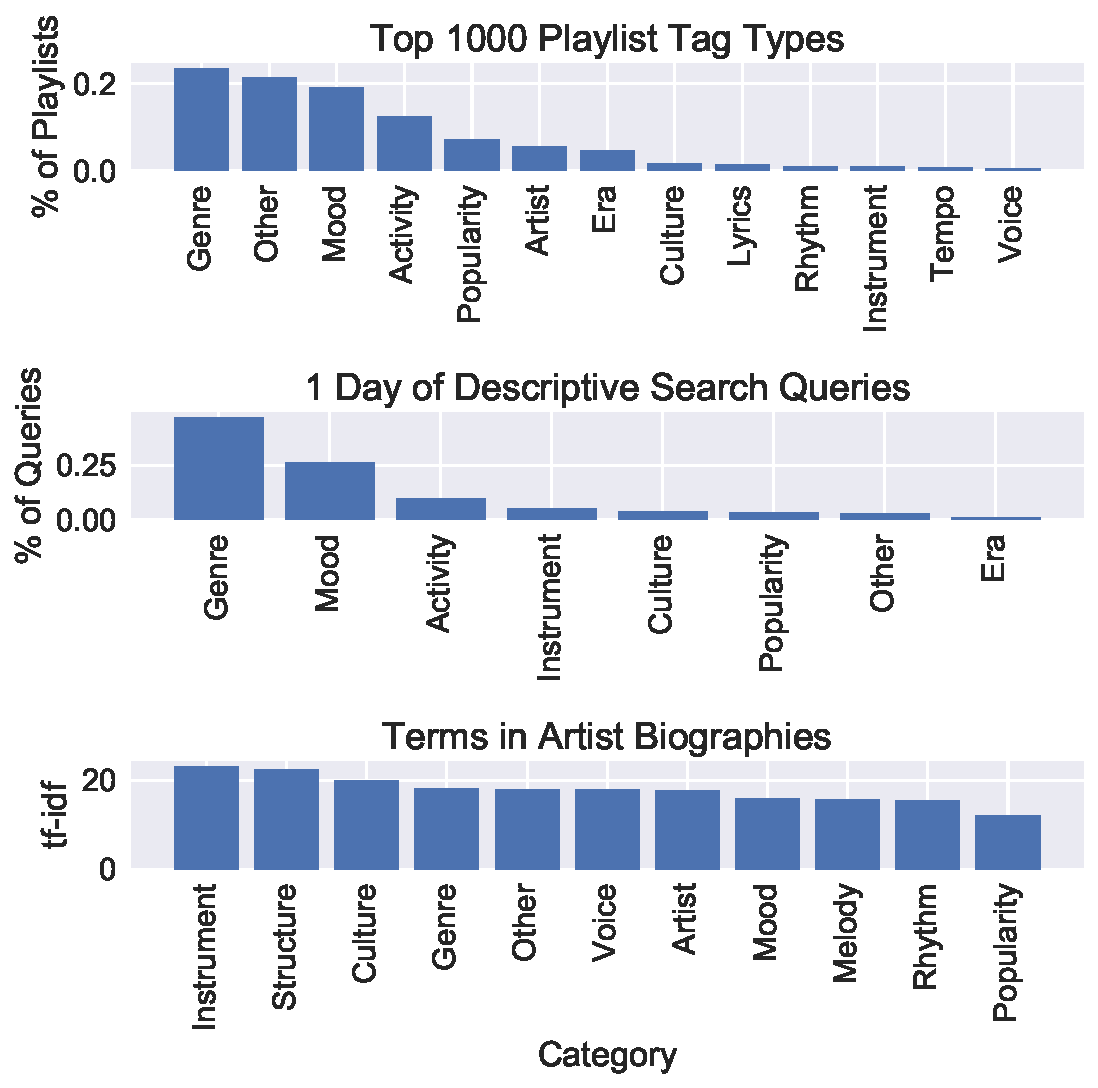
\includegraphics[width=\columnwidth]{figs/AllFreqs.pdf}
\end{center}
\caption{(Top) Percentage of Spotify playlists containing one of the top 1000 tags corresponding to each category. (Middle) Percentage of descriptive search queries corresponding to each tag category, sampled from one day of search data. (Bottom) tf-idf for each term category in artist biographies compared with Wikipedia term frequencies.}\label{fig:playlist-tags}
\end{figure}

% \begin{figure}
% \begin{center}
% 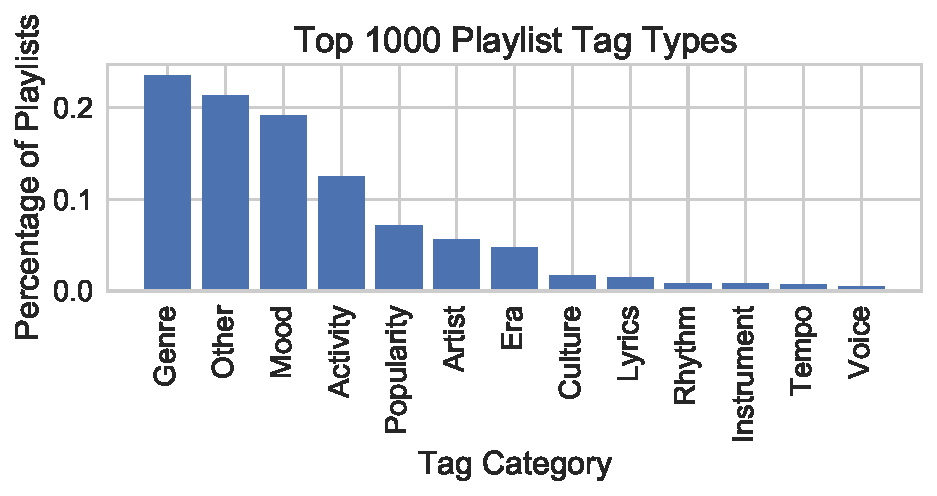
\includegraphics[width=\columnwidth]{figs/PlaylistTags.pdf}
% \end{center}
% \caption{Percentage of playlists containing one of the top 1000 tags corresponding to each tag category.}\label{fig:playlist-tags}
% \end{figure}

We perform a similar analysis on descriptive terms from one day's worth of Spotify search queries, and obtained similarly inconclusive results, shown in Figure~\ref{fig:playlist-tags}, middle.

% \subsection{Search Queries}
% We perform a similar analysis on one day's worth of search queries.
% Queries determined to be descriptive in nature (e.g.~chill electronic) rather than pertaining to a specific artist, album, song or playlist, were extracted, separated into individual tags (e.g.~``chill'', ``electronic''), and grouped into categories by a professional curator.
% Note that the categories for this analysis are the same as in the playlist analysis, with categories relating to non-descriptive tags (e.g.~Artist) omitted.
% The relative percentage of tag types is shown in Figure~\ref{fig:search-queries}.
% Again, we find that vocals are not a prominent category of descriptive search tags, and that genre, mood and activity dominate.
% This suggests that when searching for music, listeners do not use vocal descriptors, but rather other more general descriptors. Similarly to playlist titles, it may be the case that the voice may be entangled in the genre and mood descriptors.
% Another factor to consider is that of entrainment - if listeners know that searching for a specific attribute of music does not return any results, they will stop searching in that way. \ad{is it worth explaining this a bit? Here's an attempt:} As such, if the information necessary to distinguish qualities of the vocals is contained in descriptors such as genre and mood, queries based on aspects of the voice may not appear.

% \begin{figure}
% \begin{center}
% 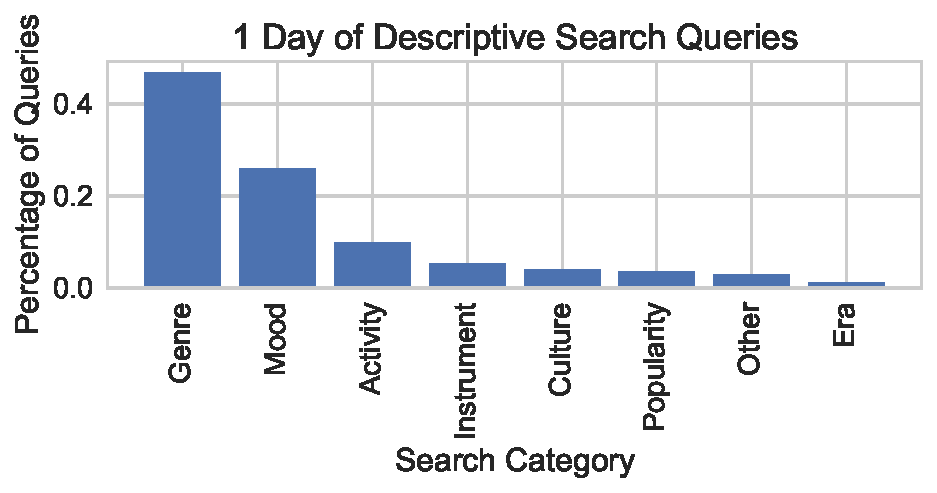
\includegraphics[width=\columnwidth]{figs/SearchQueries.pdf}
% \end{center}
% \caption{Percentage of descriptive search queries corresponding to each tag category, sampled from one day of search data.}\label{fig:search-queries}
% \end{figure}

% \rmb{People make playlists out of music they like already. Usually the group of songs is not specifically determined by the vocals???}

\subsection{Artist Biographies}

Finally, we analyze descriptive terms that occur in 100,000 professionally authored artist biographies on Spotify.
We use TF-IDF~\cite{sparck1972statistical} to retrieve terms that are distinctive to music writers, by comparing the frequency of terms in artist biographies to the frequency of the same terms in Wikipedia.
The 100 most distinctive terms, grouped into semantic categories, are displayed in Figure~\ref{fig:playlist-tags}, bottom.
While many terms are much more frequent in music text (e.g.~``bassist'', ``jazz'', ``songwriter''), vocals specifically were not more frequently mentioned than other musical aspects.
One can hypothesize that the TF-IDF method is insufficient for this particular task, due to vocals being commonly discussed outside the context of music, and thus a relatively more common word in Wikipedia.

\subsection{Conclusions}

Our results thus far do not show support for our general hypothesis. It may be the case that the intuitive notion of the relevance of vocals to user preference is misleading. On the other hand, it may also be the case that the importance of vocals is implicit in this data, as certain vocal styles are indicative of genre or mood. As such, the overlap between the voice and a number of the tags and descriptors analyzed prevents us from disentangling the unique effect of the voice from other musical components.

\section{Vocals in Survey Data}

In order to disentangle the unique effect of the voice among other components, we gathered explicit data from users.
Specifically, we conducted two online survey studies in order to collect self-reported data on 1) the salient components of music, and 2) their relative ranking. Unlike prior surveys, such as \cite{lesaffre2008potential} that presented users with short musical excerpts and groupings of adjectives to rate, we allowed the users to freely enter their responses to the question "When you listen to music, what things about the music do you notice?". This allowed us to assess whether vocals would emerge as a salient component of music. In addition, we explored what aspects of the voice users report as being important to their musical taste.

\subsection{Survey 1: Semantic Components of Music}

The aim of our first survey was to establish an unranked set of self-reported salient components of music.
While our hypothesis was that the vocals would be prominent, it was crucial to avoid biasing respondents as the data collected were explicit.
As such, our first survey asked participants what they notice when listening to music that might make them like or dislike a song. We deliberately did not specify anything further, such as the type of music, or that we were interested in components of music, nor were participants asked to listen to musical excerpts so as not to bias responses.
As an exploratory measure, we then asked participants to describe what about vocals specifically might make them like or dislike a song \textit{after} the previous open ended questions, so as not to bias responses.
Responses to these two open-response questions were manually sorted into semantic categories by the researchers. %To ensure that manual groupings were not tainted with human bias, we performed automated textual analysis on the same survey data.

\subsubsection{Recruitment}
A random sample of 50,000 people was drawn from the database of Spotify's Monthly Active Users (MUAs), divided approximately equally between the United States and Canada. 860 individuals responded to the survey, however 224 did not respond to any questions beyond the consent form, and 9 were removed for giving nonsensical responses. 626 individuals --- 338 women (average age 33.6 years with a standard deviation of 16.1); 288 men (average age 30.6 years with a standard deviation of 15.5) --- completed the survey in its entirety.

\subsubsection{Survey}
An online consent form was first presented to respondents. We then asked:

{\small
\begin{quote}
  \emph{Q1:} When you listen to music, what things about the music do you notice? Please list as many as you can think of here:
\end{quote}
}
The respondents were shown a screen with open-response format fields to complete, in which they could complete up to seven fields.
On the following screen, respondents were presented with a list of their responses in random order, and asked:

{\small
\begin{quote}
  \emph{Q2:} Please rank how important the aspects you listed are to your musical preference, where 1 is the most important.
\end{quote}
}

%The rankings were used by the research team to derive semantic categories (see below).
They were then asked the following two questions about the items they ranked from 1 to 3:

{\small
\begin{quote}
  \emph{Q3:}  (a) What about \_\_\_\_ would make you like a song? (b) What about \_\_\_\_ would make you dislike a song?
\end{quote}
}

Lastly, to explore what aspects of vocals may be relevant, participants responded to the following:

{\small
\begin{quote}
  \emph{Q4:} (Please ignore these questions if you've already mentioned the vocals, the voice, the singer/rapper etc.)
  (a) When would vocals make you like a song? (b) When would vocals make you dislike a song?
\end{quote}
}

They were then given the opportunity to comment on the survey, and were shown a final debriefing screen.

\subsubsection{Semantic Categorization}
% \subsubsection{Card sorting}
A number of partially completed surveys contained responses sufficiently complete for card sorting. 317 sufficient responses --- 262 from the completed surveys as well as 55 sufficiently complete partial -- were then card-sorted by a team of researchers.
Card-sorting is a common technique used in social sciences and elsewhere to discover clusters of related concepts~\cite{miller1969psychological}.
Traditionally, individuals are presented with physical paper ``cards'' that have terms and/or descriptions printed on them, printed pictures, or a group of objects.
They are then asked to group items in a way that makes sense, given the research question. Here, we apply card-sorting to derive semantically meaningful groupings of musical components from the freely entered words and phrases that participants entered in each field.

Participant responses to \emph{Q1} (i.e.~``When you listen to music, what things do you notice?'') were printed twice, once next to their response to \emph{Q3a} (``What about \_ would make you like a song?''), and again next to the response to \emph{Q3b} (``What about \_ would make you dislike a song?''). As such, researchers had respondents' top 3 terms printed out twice, once next to the positive descriptive aspects of the term, and once next to the negative descriptive aspects.
A term (e.g.~``the lyrics'') and its descriptor (e.g.~``when they have meaning'') comprised a card. Figure~\ref{fig:card-examples} shows examples of positive and negative cards that were used in card sorting.

\begin{figure}
\begin{center}
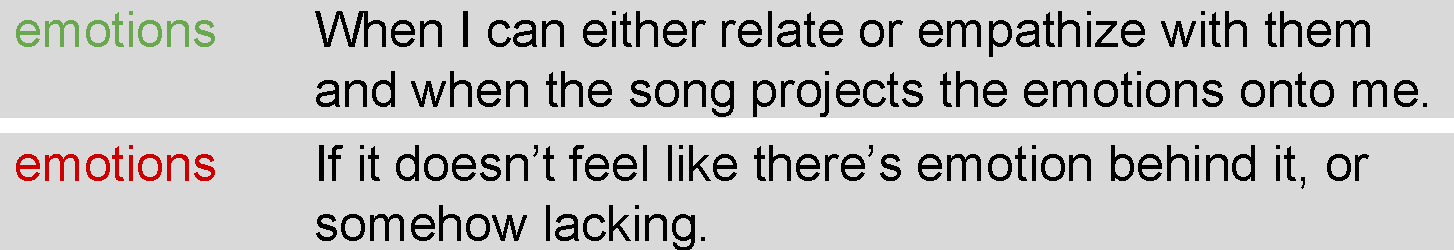
\includegraphics[width=\columnwidth]{figs/cards.pdf}
\end{center}
\caption{Survey 1 sample answers for \emph{Q3}. (Top) Card for an answer to \emph{Q3a}. (Bottom) Card for an answer to \emph{Q3b}.}
\label{fig:card-examples}
\end{figure}

% \begin{figure}[t!]
%     \centering
%     \begin{subfigure}[t]{0.5\textwidth}
%         \centering
%         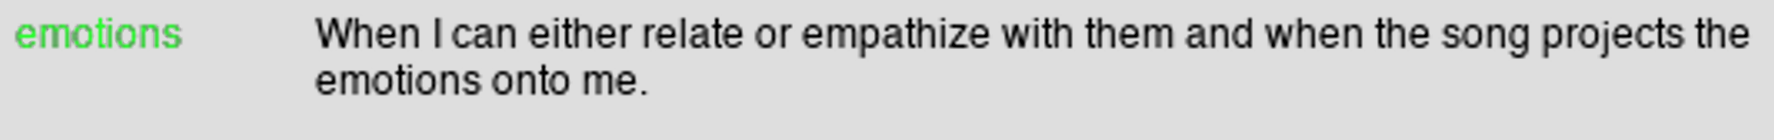
\includegraphics[width=\columnwidth]{figs/card-positive.png}
%         \caption{Card for an answer to \emph{Q3a}}
%     \end{subfigure}

%     \begin{subfigure}[t]{0.5\textwidth}
%         \centering
%         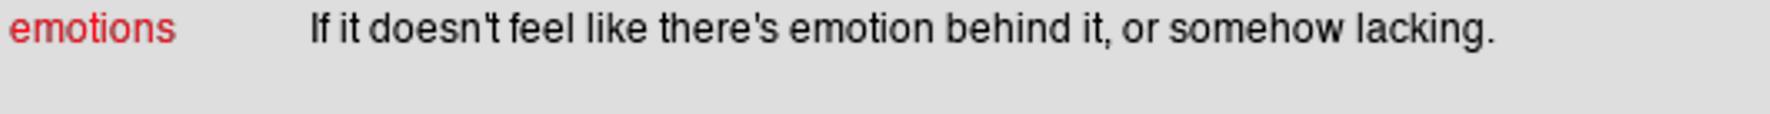
\includegraphics[width=\columnwidth]{figs/card-negative.png}
%         \caption{Card for an answer to \emph{Q3b}}
%     \end{subfigure}
%     \caption{Example sorting cards}
%     \label{fig:card-examples}
% \end{figure}

As some responses were unclear (e.g.~``the melody'' was mentioned, but the descriptor clearly focused on the quality of the singer's voice), the research team was instructed to look at both the term and its descriptor when determining its semantic category.
The researchers then reviewed the cards a second time, and defined sub-categories where necessary.

%% \rmb{I moved all of this down to results, I think it flows better as one block}
% \subsubsection{Natural Language Processing}
% In order to validate that the semantic categories derived via card-sorting were not affected by our biases, we also quantified the categories by computing word counts.
% Simple natural language processing (NLP) was used to quantify the categories in survey responses.
% The text from responses was parsed into independent words, aggregated and counted.
% Common words were removed such as ``it'', ``like'', ``sometimes'', or ``when'', and similar words were combined such as ``drum'' and ``drums'' or ``voice'' and ``vocals''.
\subsubsection{Results}

The output of this study was two sets of semantic categories: broad semantic categories of music, and vocal-specific semantic categories.
Statistical testing was not possible, given the intentionally imprecise nature of the responses.
However, out of the 626 responses to the first question, 186 (29.7\%) mentioned the vocals, the voice, or the singer, 348 (55.6\%) mentioned the lyrics, or the words, and 101 (16.1\%) mentioned both. While this is no indication of relative importance, it does demonstrate that the voice and the lyrics were salient musical components to our respondents.

The broad semantic categories determined by the researchers are presented in the left column of Table~\ref{tab:mus-attributes} (note that the other results in Table~\ref{tab:mus-attributes} are from Study 2).
The category of \textit{Emotion/mood} referred to the ability of a song to evoke emotion, whether the emotion was a match or a mismatch to the current or desired mood or current activity, whether the emotion was desirable or undesirable, and nostalgia.
\textit{Voice} included genre related terms (e.g.~mumble rap, metal, auto-tune, speechiness/rapping), descriptions of how the voice is used (e.g.~unique/novel, screaming, pitch/pitch range, presence or absence of effects, intensity/effort/power, emotionality, authenticity, whininess/nasality, melodic-ness), skill, the innate qualities of the voice, liking/disliking, and the mix/blend.
The \textit{Lyrics} category represented items that indicated whether or not lyrics were present, their intelligibility, the presence of profanity, how ``well'' crafted they were, the ``message'', the meaning behind them or general lyrical content and how relatable they are.
\textit{Beat/Rhythm} referred to whether it was liked/disliked, whether it ``fit'' the song, danceability, and uniqueness.
The \textit{Structure/complexity} of songs included liking or disliking the hook or chorus, and the song length.
Instrumentation referred to drums, bass, and guitar.
\textit{Sound} referred to audio quality and related concerns.
Self-explanatory categories included \textit{Tempo/BPM}, the mention of a \textit{Specific Artist}, \textit{Genre}, \textit{Harmony}, \textit{Chords}, \textit{Musicianship}, \textit{Melody}, and \textit{Popularity/Novelty}.

% \subsubsection{Quantifying Semantic Categories}

% In order to roughly quantify the frequency with which each type category was mentioned,the text from responses was parsed into independent words, aggregated and counted.
% Common words were removed such as ``it'', ``like'', ``sometimes'', or ``when'', and similar words were combined such as ``drum'' and ``drums'' or ``voice'' and ``vocals''.
% The categories from this analysis were compared against our defined categories, and the results are shown in Figure~\ref{fig:category-count}.

% \begin{figure}
% \begin{center}
% 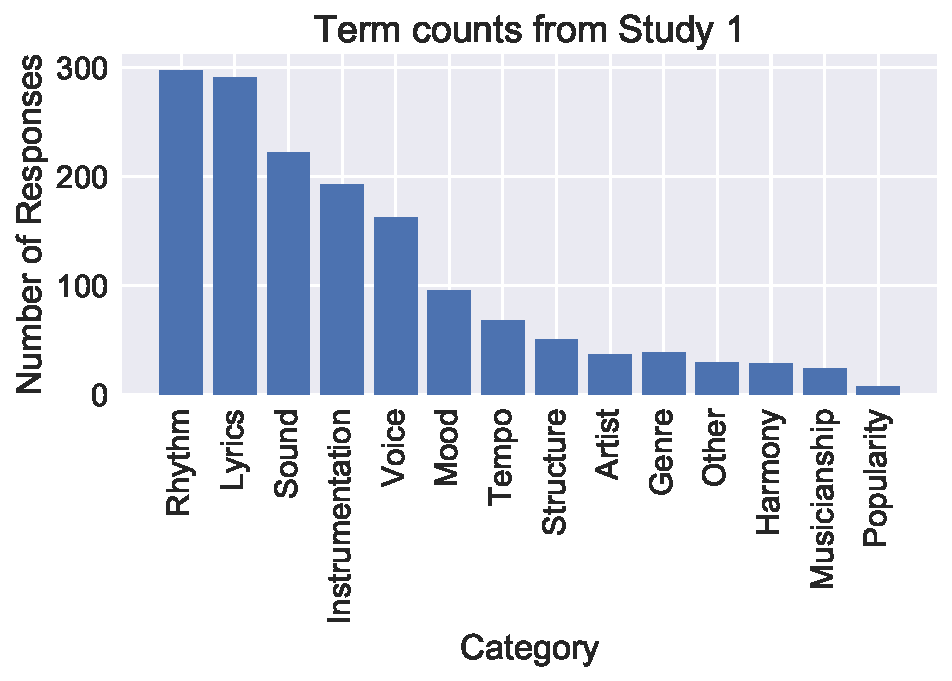
\includegraphics[width=\columnwidth]{figs/Survey1_frequencies.pdf}
% \end{center}
% \caption{Number of responses for survey categories.}
% \label{fig:category-count}
% \end{figure}

%The NLP categories were mapped to card sorting groups.
%Then the terms were counted, where each term could be counted once for each person.  The results are in figure X.
% It is interesting to note that the most commonly mentioned terms involved the "voice", "lyrics" and "vocals".
% This was an open ended survey where people could respond in any way.
% The participants were not primed or restricted to respond according to any specific categories.
% \aj{is this redundant given the numbers we give in the above Results subsubsection?}

\subsection{Survey 2: Component Ranking}

While the first study aimed at determining what attributes of music were salient in the minds of listeners, the aim of the second survey was to determine the relative importance of each of the components. Specifically, we explored whether the voice would be ranked highest among a list of musical attributes.
To accomplish this, participants were asked to rank a list of attributes derived from the results of our first survey, thus allowing an assessment of whether or not vocals rank above other components.

%\subsubsection{Methods} %% [AJ] let's scrap this level

\subsubsection{Recruitment}
A randomized sampling method was employed among the database of Spotify's Monthly Active Users (MAUs) that had not opted-out of email correspondence.
An email with a link to an online survey was sent to 50,000 potential respondents, approximately equally divided among the United States and Canada.
%\aj{Can this and the survey 1 recruitment sections be collapsed into one somehow?}

A total of 531 respondents --- 263 of which were women (average age 31.8 years, with a standard deviation of 16.5); 268 were men (average age 34.2 years, with a standard deviation of 14.8) --- completed the survey in its entirety. 429 participants completed the first half of the survey (broad semantic categories), whereas 360 participants completed the second half (vocal semantic categories).

\subsubsection{Survey}
An online consent form was first presented to respondents.
The derived semantic categories were rephrased to be more easily understood (see Table~\ref{tab:mus-attributes}, Description).
Participants were presented with the new list of descriptions in random order, and asked to ``Please click all the items below that would make you like or dislike a song.'' They were then presented with a list of all the items they had clicked, also in random order, and asked to rank them.

\begin{table*}[h!]
\begin{center}
\rowcolors{1}{white}{gray!25}
\begin{tabular}{ l  l  r  r }
\hline
\textbf{Broad Semantic Category} & \textbf{Description} &\textbf{Borda score} & \textbf{$p$-value}\\
\hline
Emotion/mood & How it makes you feel - the emotions/mood & 4641 & \textbf{\textless 0.001}\\
Voice & Voice/vocals & 3688 & \textbf{\textless 0.001}\\
Lyrics & Lyrics & 3656 & \textbf{\textless 0.001}\\
Beat/rhythm & Beat/rhythm & 3460 & \textbf{\textless 0.001}\\
Structure/Complexity & How it's composed, the hook, the structure & 2677 & 1.000\\
Musicianship & Skill of the musicians, musicianship & 2583 & 1.000\\
Melody & The main melody & 2577 & 1.000\\
Sound & The ``sound'', or the recording quality & 2406 & 1.000\\
Specific Artist & The specific artist & 2349 & 1.000\\
Genre & The specific genre & 2293 & 1.000\\
Instrumentation & The musical instruments (e.g.~drums, bass, guitar) & 2084 & 1.000\\
Tempo/BPM & How fast or slow the song is & 1828 & 1.000\\
Harmony & Harmony & 1763 & 1.000\\
Chords & The chords & 1086 & 1.000\\
Popularity/Novelty & How popular or unique it is & 777 & 1.000\\
\hline
\end{tabular}
\end{center}
\caption{Broad semantic categories and their clarifying descriptions created during Study 1, ordered by rankings from Study 2 (see Study 1 results for attribute descriptions). The Borda scores and $p$-values from Study 2 are reported in columns 3 and 4. Statistically significant $p$-values are shown in bold. $p$-values of 1.000 indicate that the ranking is no different from random.}
\label{tab:mus-attributes}
\end{table*}

As a continuation of our exploratory study of vocal characteristics, a second list was then presented, comprised of terms derived from the vocal and lyrics semantic categories.
For clarity, the terms were rephrased as they appear in Table~\ref{tab:voc-attributes}.

\subsubsection{Analytic Strategy}
Responses were subjected to Borda counting \cite{Borda1781} and Robust Rank Aggregation \cite{kolde2012robust}.
Borda counting is a simple procedure for aggregating votes by summing ranks.
The Borda score $B_i$ for an item $i$ is computed as
$B_i = \sum_{p=0}^N \left( |r_p| - r_{p, i} \right)$
where $N$ is the number of participants, $r_{p,i}$ is participant $p$'s rank of item $i$, starting at zero, and $|r_p|$ is the number of items ranked by $p$.
The Borda method does not naturally extend to partial lists\cite{dwork2001rank} --- we have chosen to award higher scores to preferred items in long lists.

To verify the statistical significance of our findings we supplement the Borda count with Robust Rank Aggregation (RRA), in which we compare our survey results to a null hypothesis.
Each item receives a score based on its observed position, compared to an expected random ordering.
Upper bounds to $p$-values are computed using Bonferroni correction, with values of 1.0 indicating null findings.
In this work we used the implementation provided by the \textsc{RobustRankAggreg} package\footnote{\url{cran.r-project.org/web/packages/RobustRankAggreg}}.

\subsubsection{Results and Conclusion}

Results can be found in Tables \ref{tab:mus-attributes} and \ref{tab:voc-attributes}, with categories ordered by descending Borda count.
We are able to show statistical significance of both the most salient broad and vocal semantic categories.
Importantly, our results show that the Vocals and Lyrics ranked second and third among the list of components (Borda scores and RRA agree on the order of the first four broad categories).
This indicates that, relative to other musical components, respondents overall indicated the importance of the vocals and lyrics.

\begin{table*}[h!]
\begin{center}
\rowcolors{1}{white}{gray!25}
\begin{tabular}{| c | l r r |}
\hline
& \textbf{Vocal Semantic Categories} &\textbf{Borda score} & \textbf{$p$-value}\\
\hline
A & Singing skill & 3423 & \textbf{\textless 0.001} \\
B & How well the voice fits or matches the rest of the music & 3380 & \textbf{\textless 0.001}\\
C & Lyrical skill / cleverness / wit & 3145 & \textbf{\textless 0.001}\\
D & The meaning, or the ``message'' of the words & 3038 & \textbf{0.048}\\
E & Authenticity / ``realness'' & 2884 & \textbf{\textless 0.001}\\
F & Uniqueness & 2780 & \textbf{\textless 0.001}\\
G & If the voice is emotional & 2771 & \textbf{0.006}\\
H & Voice strength / intensity / effort & 2721 & 1.000\\
I & If the voice sounds natural & 2480 & 1.000\\
J & Being able to relate & 2256 & 1.000\\
K & If the voice is melodic & 2202 & 1.000\\
L & Whether or not you can understand the lyrics & 2056 & 1.000\\
M & If it's whiny or nasal & 1801 & 1.000\\
N & Whether or not there's screaming & 1771 & 1.000\\
O & The overall pitch, or the range of the pitch & 1400 & 1.000\\
P & Whether or not there are lyrics & 1250 & 1.000\\
Q & Whether it has production effects on it, like autotune & 1230 & 1.000\\
R & Profanity, explicit lyrics & 1086 & 1.000\\
S & Whether or not there is rapping & 909 & 1.000\\
\hline
\end{tabular}
\end{center}
\caption{Vocal-specific semantic categories from Study 1, ordered by rankings from Study 2. Columns 2 and 3 show the Borda scores and $p$-values. Statistically significant $p$-values are shown in bold. $p$-values of 1.000 indicate that the ranking is no different from random.}\label{tab:voc-attributes}
\end{table*}

\section{New Avenues for Research}
While the musical attributes related to the broad musical categories (Table~\ref{tab:mus-attributes}) are well studied in MIR, the attributes related to vocals (Table~\ref{tab:voc-attributes}) present a number of exciting and unexplored research directions.
A limiting factor to studying some of these problems, as is often the case, is the availability of data, and we encourage researchers to focus data collection efforts in these areas as well. A further limiting factor is that users of online musical platforms may come from a specific demographic, e.g. regular internet users typically younger than 35, who engage in music related activities in about one third of the online time, have had at least some musical education, and have a preference for pop, rock and classical music \cite{lesaffre2008potential}. In addition, our sample was derived from the U.S. and Canada. As such, a cross-cultural sample may differ in their relative preference for vocals.

%% This is commented below because singing skill assessment is pretty well studied from a cursory google search
% Singing skill assessment has been studied in the context of education~\cite{}, karaoke~\cite{tsai2012automatic} and in general~\cite{gupta2017perceptual}.
% An interesting new research direction would be to measure the singing skill of a singer in recorded music, possibly based on characteristics of the singer's pitch, timbre, and articulation.

Our exploratory data suggest that there is a vast space of research in tagging and measuring different qualities of the singing voice, such as whether a singing voice is authentic, powerful, natural, melodic, nasal, or emotional (Table~\ref{tab:voc-attributes}, rows E, H, I, K, M and G).
In addition to these categories, determined by untrained listeners, there are a number of other more specific categories such as modes of phonation that could be explored. %are used commonly by music critiques.
%For example, Table~\ref{tab:album-reviews} shows a collection of terms commonly used to describe vocals drawn from a large collection of album reviews, each of which would be interesting to model.
Further, in addition to vocal qualities, there are genre-centric vocal styles, such as identifying rap or screaming (Table~\ref{tab:voc-attributes}, rows S and O).

% \begin{table}
% \begin{center}
% \rowcolors{1}{gray!25}{white}
% \begin{tabular}{| c | c | c | c | c |}
% \hline
% lead & backing & powerful & clean & beautiful \\
% haunting & smooth & ethereal & soaring & dreamy\\
% sweet & layered & soft & breathy & sultry\\
% angelic & deep & falsetto & delicate & raspy\\
% \hline
% \end{tabular}
% \end{center}
% \caption{Common adjectives used to describe vocals in album reviews.}\label{tab:album-reviews}
% \end{table}

Another interesting and (as far as we are aware) unexplored research area is to measure whether a voice fits or blends well with the background music (Table~\ref{tab:voc-attributes}, row B).
This is somewhat related to the problem of determining ``mashability'' in automatic-mashup generation.
This is a broad problem that is likely based on many factors, such as the style of the vocalist compared to the background, the way the song is mixed, and the overall expectations of the musical genre.
We suspect this could be most easily studied when isolated vocals/backgrounds are available in order to automatically generate examples of vocals that do not match the background by blending random combinations.

The problem of identifying whether a voice is ``unique'' is likely challenging (Table~\ref{tab:voc-attributes}, row F), as it is not necessarily a quality that can be determined in isolation, but rather relative to many other voices.
One possible approach to this problem would be to treat the problem as one of outlier detection.
%Alternatively, it is possible that a listener's perception of what sounds ``unique'' is not truly unique, but rather a particular distinguishable quality.

Production effects applied to the singing voice are increasingly common, especially different types of distortion or the infamous auto-tune (Table~\ref{tab:voc-attributes}, row Q).
Automatic identification of these production effects presents an interesting challenge, and one where data could be automatically generated with the help of plugins for generating effects and databases with isolated vocals with corresponding backgrounds.

Measuring the relatability (Table~\ref{tab:voc-attributes}, row J) of a singer is a quality that is relative to the listener, rather than absolute.
Factors that could affect a singer's relatability could include the age, gender, culture or language of the singer relative to the listener, which might require automatic identification of each of these attributes of the singer.

Lyric intelligibility (Table~\ref{tab:voc-attributes}, row L) has not been well studied, and also presents a novel challenge~\cite{ibrahim2017intelligibility}.
This problem does not necessarily directly require lyric transcription, and may be able to be determined from qualities of the audio.
Similarly, determining whether a singing voice contains lyrics or is wordless has not been studied (Table~\ref{tab:voc-attributes}, row P).

Automatic lyric transcription has been studied~\cite{mcvicar2014leveraging,kruspe2016retrieval} but is not yet solved, and would power the automatic estimation of many of these vocal attributes.
For lyric-related terms, given textual lyrics, while some attributes would be relatively simple to estimate (e.g.~whether or not there is profanity), others present interesting NLP challenges, such as estimating whether the lyrics are ``clever'' or are ``meaningful'' (Table~\ref{tab:voc-attributes}, rows R, C, and D).

\section{Discussion and Conclusions}

While our analyses of playlist titles and search queries were inconclusive, we show evidence that English-speaking respondents from the U.S. and Canada clearly indicated that the voice is a salient component of music.
Specifically, Spotify users were asked what they notice about music while listening.
Despite the unassuming nature of the question, our results showed that the voice was indeed salient among the group of reported musical attributes.
Furthermore, users ranked the voice as the second most important component to their musical preference, after emotions.

Our results have a number of implications.
With regards to MIR research specifically, our results suggest that the voice and lyrics are indeed relevant attributes that warrant further study.
While individuals may not necessarily want or know how to describe vocals themselves, i.e.~in their playlists or search queries, surveying listeners directly does indicate that they find vocals to be important.
As such, clarifying how the voice relates to music preference is an important topic for future research.

Secondly, users indicated that the ability of a song to evoke emotions was the most important factor.
This confirms findings in prior research of the relevance of emotional content in music, and how it is linked to musical preference, e.g.~\cite{krumhansl2017listening}.
Therefore, examining how music affects the emotions of listeners remains an important theme.
Interestingly, while genre was the most frequent term used to label playlists or search for music, respondents did not rank the specific genre as important relative to the other attributes.
Understanding why this is the case warrants further study.

More relevant to our hypothesis, is that the vocals and the lyrics of a song were ranked second and third by respondents who were directly asked what components of music are important to their preferences.
Therefore the link between emotions perceived in the voice and lyrics, and the emotions felt in listeners, is very relevant to questions of music preference.
Clarification of these links was out of scope in these studies, and could be addressed in future research.

Lastly, we show the relevance of explicitly collected data that might guide future research.
While we showed inconclusive findings regarding the prevalence of vocals in implicit data, we did show that the unique effect of vocals on music preference may be observed using survey data.
As such, explicit data-gathering techniques often found in the social sciences, as well as collaborations with social scientists, may be of great use to MIR researchers.


% For bibtex users:
\bibliography{references}

\end{document}
